\chapter{Calibration}
In the process of combining data from several view points, a model of the system is needed as to align the measurements correctly. An idealised model can be formulated based on motion theory, but in inherently imperfect hence the need for calibration. In the context of eye-in-hand based surface reconstruction, especially calibrating the kinematic chain from object robot base is important in order to combine data from several views. Calibration of robot systems has received considerable attention and continues to be an active field of research. A solution for the unknown transforms from camera to end effector and from object to robot base can be obtained relatively easy by solving a homogeneous transform \cite{Shiu1989}. Several algorithms for more or less autonomous calibration has been proposed \cite{Tsai1988, Tsai1989} often simultaneously calibrating camera and hand-eye \cite{Malm2003, Zhao2008, Jordt2009}. The calibration process presented here is based on the linear method \cite{Tsai1988} with some application specific modifications.


\section{Notation}
In the formulation of hand-eye calibration a number of homogeneous transforms between frames are be described. Most literature uses a mathematically founded notation of \textit{Ai}, \textit{Bi}, \textit{A}, \textit{B}, \textit{X} and \textit{Y} leading to nice and clean equations. In this work a more explicit and engineering friendly notation will be used stating for each transform the state index (since there are several different robot states involved to allow different views of the object), the name of the frame described and the name of the reference frame. Examples of the notation are explained in table \ref{tab:notation}. The transform is a a 4x4 matrix containing a 3x3 rotation matrix and a 1x3 translation vector. The terms end-effector and Tool Center Point(TCP) will be used interchangeably.\\

\begin{table}[h]
\caption{Examples of the notation used to describe rigid transformation.}
\begin{tabular}{ll}
\label{tab:notation}
$[T_{i}]_{camera}^{object}$   & The transform from object to camera at the \textit{i}th robot state          \\[8pt] 
$[T_{i}]_{base}^{TCP}$        & The transform from end-effector to base at the \textit{i}th robot state      \\[8pt] 
$[T_{i}]_{TCP}^{camera}$      & The transform from camera to end-effector at the \textit{i}th robot state     \\[8pt] 
$[T_{i-1,i}]_{camera}$        & The camera frame at state \textit{i} relative to the camera frame at state \textit{i-1}  \\[8pt]              
\end{tabular}
\end{table}

\begin{figure}[htb]
	\begin{center}
		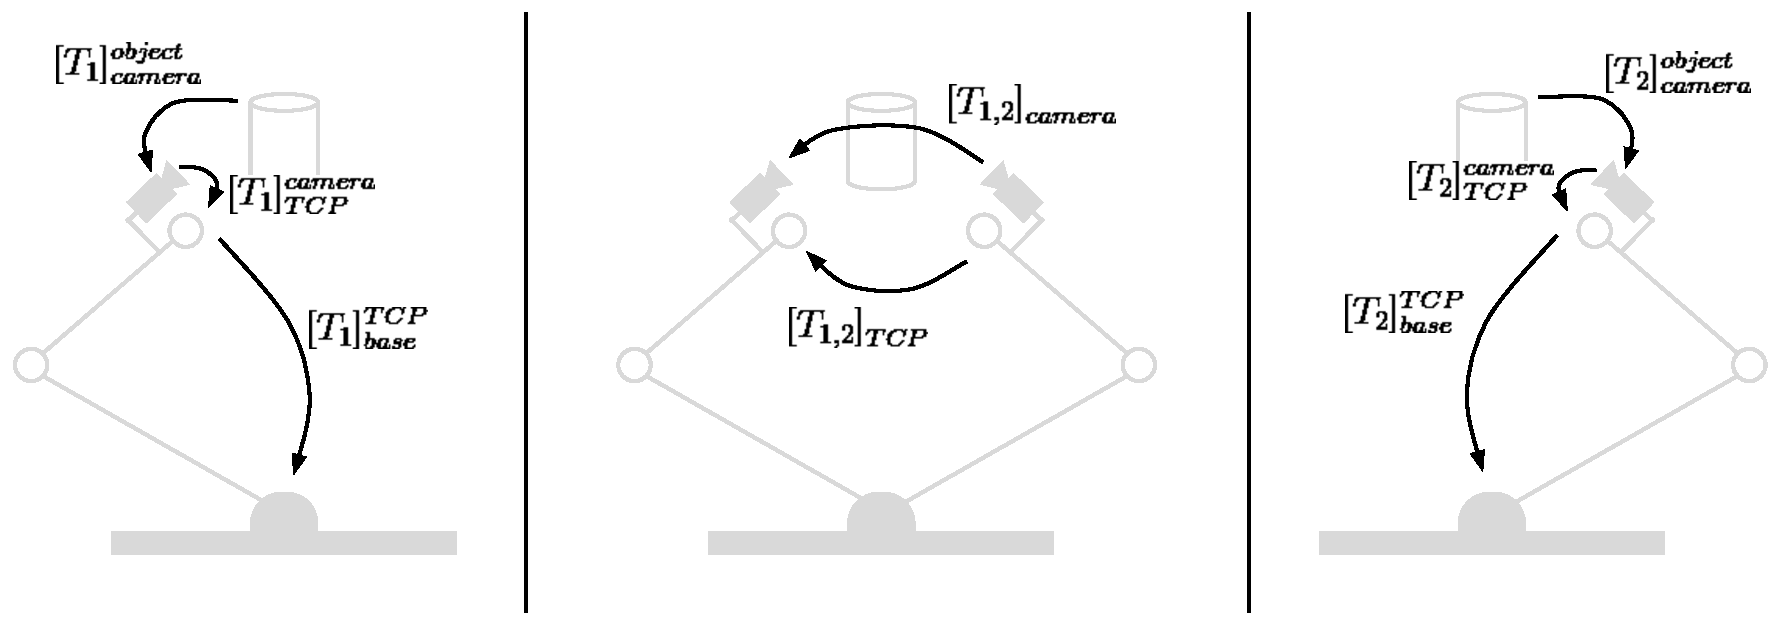
\includegraphics[width=\textwidth,trim=0 0 0 0]{graphics/03_calibration/hand_eye_transforms.pdf}%trim=l b r t
		\caption{Sketch of a robot with a camera mounted on the end-effector in two different states capturing a cylinder object. Shows the robot in state 1 (left), state 2 (right) and both robot states in same image (center).}\label{fig:hand_eye_transforms}
		
	\end{center}
\end{figure}

\section{Linear hand-eye calibration}
\noindent Looking at figure \ref{fig:hand_eye_transforms} (left and right) it is clear that a kinematic chain from the object to the robot base can be formulated.\\

\begin{equation}
	[T_{i}]_{base}^{object} = [T_{i}]_{base}^{TCP} \cdot [T_{i}]_{TCP}^{camera} \cdot [T_{i}]_{camera}^{object}
\end{equation} \\

\noindent The transform from end-effector to robot base can be found from the joint states of the robot and the transform from object to camera can, assuming the camera is calibrated, be found from projection geometry. This leaves only the transform from camera to end-effector as unknown. Assuming that the object is static and captured from different robot states, it is possible to formulate the transform between the two camera poses (Figure \ref{fig:hand_eye_transforms}, center).\\

\begin{equation}\label{eq:object_camera}
\begin{matrix}
[T_{1,2}]_{camera} \cdot [T_{1}]_{camera}^{object} = [T_{2}]_{camera}^{object} \\
\\  
\Updownarrow \\ 
\\ 
[T_{1,2}]_{camera} = [T_{2}]_{camera}^{object} \cdot ([T_{1}]_{camera}^{object})^{-1}
\end{matrix}
\end{equation}\\ 

\noindent Similarly the transform between the two poses of the end-effector can be formulated(\ref{fig:hand_eye_transforms}, center).\\

\begin{equation}
\begin{matrix}
[T_{1}]_{base}^{TCP} \cdot [T_{1,2}]_{TCP} = [T_{2}]_{base}^{TCP} \\ 
\\ 
\Updownarrow \\ 
\\ 
[T_{1,2}]_{TCP} = ([T_{2}]_{base}^{TCP})^{-1} \cdot  [T_{1}]_{base}^{TCP}
\end{matrix}
\end{equation}\\ 

\noindent Assuming that the transform from camera to end-effector is static it is clear that.\\

\begin{equation}
[T_{1}]_{TCP}^{camera} = [T_{2}]_{TCP}^{camera} = [T]_{TCP}^{camera}
\end{equation}\\ 

\noindent This makes it possible to formulate a closed loop kinematic chain (\ref{fig:hand_eye_transforms}, center). This equation is in most literature denoted $ AX=XB $. \\

\begin{equation} \label{equ:closed_loop}
	[T_{1,2}]_{camera} \cdot [T]_{TCP}^{camera} = [T]_{TCP}^{camera} \cdot [T_{1,2}]_{TCP}
\end{equation}\\ 

\noindent The missing transform can thus be found by solving a set of $ n-1 $ linear equations for $ n $ robot states \\

\begin{equation} \label{eq:linear_equations}
\left\{\begin{matrix}
[T_{1,2}]_{camera} \cdot [T]_{TCP}^{camera} = [T]_{TCP}^{camera} \cdot [T_{1,2}]_{TCP} \\ 
\ \ \vdots 
\\ 
[T_{i-1,i}]_{camera} \cdot [T]_{TCP}^{camera} = [T]_{TCP}^{camera} \cdot [T_{i-1,i}]_{TCP}\\ 
\ \ \vdots 
\\ 
[T_{n-1,n}]_{camera} \cdot [T]_{TCP}^{camera} = [T]_{TCP}^{camera} \cdot [T_{n-1,n}]_{TCP}
\end{matrix}\right.
\end{equation}\\ 

\noindent Normally the calibration is made by capturing views of a chessboard marker from several robot states. There are however two rather implicit assumptions \cite{Horaud1995} not justified by this approach. First the calibration of the camera assumes a perfect pinhole model and that the optical axis of the camera is perpendicular to the object, but equation \ref{equ:closed_loop} assumes that the object is static, which for most practical objects are contradictions. There are several approaches to solving this, but those are outside the scope of this discussion. 

\section{Application specific method}
In this work an alternative approach is taken to include more of the possible uncertainties in the hand-eye calibration and to account for the unjustified assumptions mentioned above. Uncertainties in the vision process generating the transform from object to camera could stem from inaccurate parameters, the pinhole model assumption or pixel quantisation errors to mention a few. Uncertainties in the transform from end-effector to base can stem from mechanical inaccuracies, wear and tear, quantisation errors in encoders or from dynamics, also just to mention a few. \\

\noindent Solving the linear system from equation \ref{eq:linear_equations} is equivalent to making a least-squares fit and thus after calibration a fixed transform minimising the error over all robot states is applied to each state. The problem with this is that a linear method is used to estimate errors that are by no means linear. Furthermore the method is vulnerable to outliers, since one faulty view will influence all others. Instead a method capable of fitting non-linear functions is desirable, but to use such, individual errors at each robot state must be known. Furthermore it is desired to include as much of the reconstruction process as possible inside the the calibration loop, to account for as many errors as possible. Therefore it is desirable to base the calibration on the point clouds instead of the camera output and furthermore it is desirable to evaluate each data pair instead of pooling them for all views.\\

\noindent Estimating a rigid transform between two point clouds is considered an absolute orientation problem \cite{Horn1987} and can be solved with an Iterative Closest Point(ICP) algorithm. The ICP algorithm tries to estimate a transform to align the source cloud to the target cloud by alternating between matching points that are close, estimating the transform and transforming the remaining points. Normally the transform is estimated using least-squares, but an alternative implementation using damped least-squares\cite{Gavin2011} and thus not assuming linearity is found in PCL (\texttt{pcl::IterativeClosestPointNonLinear< \ldots , \ldots >}). This is already implemented as part of the point cloud registration process is the modelling component where it is used for pairwise alignment of the point clouds as part of the registration process. Knowing the pairwise pose estimate means that another closed loop formulation can be expressed (Figure \ref{fig:new_calibration}). \\

\noindent Taking as example the camera pose at state 1 ($ [T_1]_{base}^{camera} $) and following the pairwise alignment transforms all the way around ending up back at state 1 the result must be equal to the original pose and the error at that pose.

\begin{equation}
\begin{matrix}
[T_{1}]_{base}^{camera} \cdot [T_{12}]_{PC} \cdot [T_{23}]_{PC} \cdot [T_{34}]_{PC} \cdot [T_{45}]_{PC} \cdot [T_{51}]_{PC} = [T_{1}]_{base}^{camera} \cdot [T_{1}]_{camera}^{error}
\\ 
\Updownarrow \\ 
\\ 
[T_{12}]_{PC} \cdot [T_{23}]_{PC} \cdot [T_{34}]_{PC} \cdot [T_{45}]_{PC} \cdot [T_{51}]_{PC} = [T_{1}]_{camera}^{correction}
\end{matrix}
\end{equation}\\ 

\noindent Looking at the closed loop in figure \ref{fig:new_calibration} if say the view at state 3 had a large error, that error would in the evaluation of all other states result in two contributions ($ T_{23} $ and $ T_{34} $) of equal magnitude and opposite sign. This means the method is robust to outliers. Now having estimated the error at each pose, a non-linear method can be used to estimate the calibrated transform. The ideal method would be one eliminating the error in each state, while interpolating in between. However such a method cannot be made with a static transform.\\

\noindent The final calibrated transform from end-effector to camera $[T]_{TCP}^{camera}$ is composed of the transform from the a priori 3D model of the robot and a correction transform. \\

\begin{equation}
[T]_{TCP}^{camera} = [T_{model}]_{TCP}^{camera} \cdot [T_1]_{camera}^{correction}
\end{equation}\\

The correction transform $[T_1]_{camera}^{correction}$is obtained by multiplying the error at each pose. \\

\begin{equation}
[T_1]_{camera}^{correction} = [T_2]_{camera}^{correction} \cdot [T_3]_{camera}^{correction} \dots [T_n]_{camera}^{correction}
\end{equation}\\

\begin{figure}[htb]
	\begin{center}
		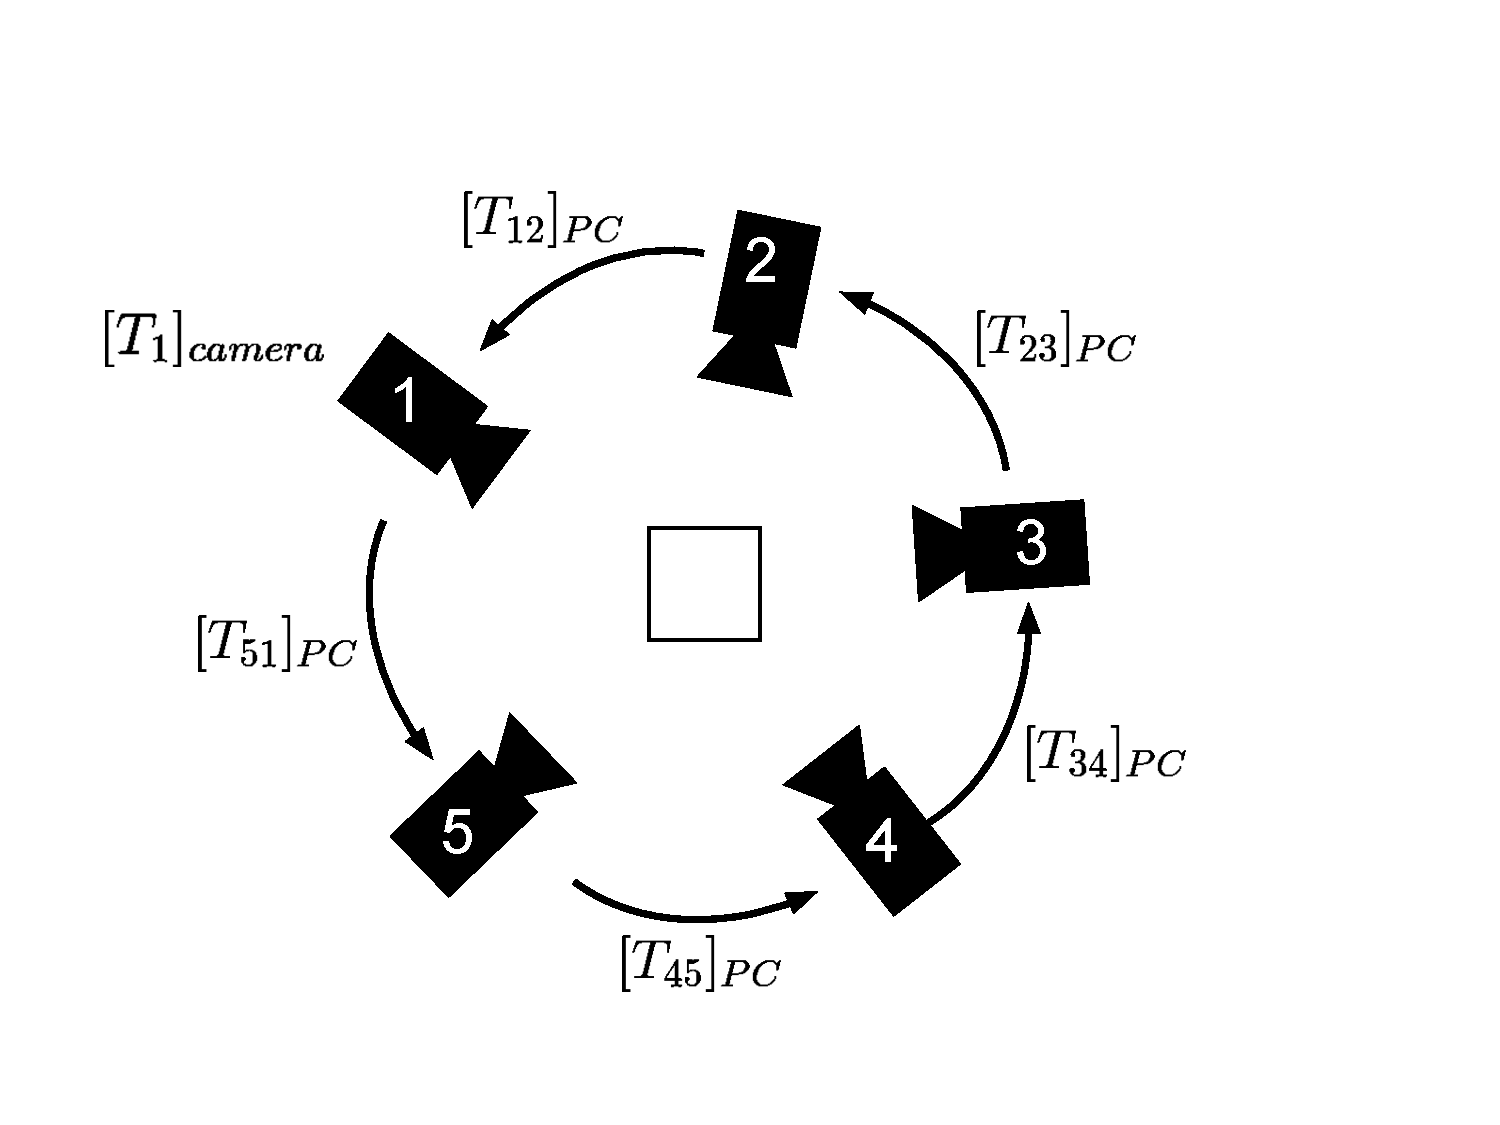
\includegraphics[scale=0.4,trim=0 0 0 0]{graphics/03_calibration/new_calibration.pdf}%trim=l b r t
		\caption{The closed loop formed by the point cloud transformations.}\label{fig:new_calibration}
	\end{center}
\end{figure}


 



